\documentclass[12pt]{article}
\usepackage{amssymb,amsmath,amsthm,mathtools}
\usepackage{hyperref,cleveref}
\usepackage[margin=1.25in]{geometry}
\usepackage{graphicx,ctable,booktabs} 
\usepackage[parfill]{parskip} % begin paragraphs on empty line rather than indent
\usepackage{fancybox}
\usepackage{tipa} % for \textpipe
\usepackage{caption}
\usepackage{subcaption}
\usepackage{bbm}

\usepackage{tikz}
\usetikzlibrary{shapes,arrows,positioning}

\setlength{\parindent}{1cm}
\usepackage{epstopdf} % eps to pdf, declare graphics
\usepackage{soul} % enable highlighting text: use \hl{your text here}
\DeclareGraphicsRule{.tif}{png}{.png}{`convert #1 `dirname #1`/`basename #1 .tif`.png}
\def\thesection{\arabic{section}} % adjust section and subsection labelling 
\def\thesubsection{\arabic{section}(\alph{subsection})}
\makeatletter
\newenvironment{pr}{\@startsection % section as pr
       {section}{1}
       {0.4em}{-.5ex plus -1ex minus -.2ex}{.5ex plus .2ex}
       {\pagebreak[3]\large\bf\noindent{Problem}}}
       {\nopagebreak[3]\vspace{3ex}}
\newenvironment{pa}{\@startsection % subsection as pa
       {subsection}{2}
       {0.3em}{0ex plus -1ex minus -.2ex}{.5ex plus .2ex}
       {\pagebreak[3]\large\noindent{}}}
       {\nopagebreak[3]\vspace{3ex}}
\makeatother
\usepackage{fancyhdr}
\pagestyle{fancy}
\lhead{\footnotesize Adrien Fallou} % header left
\chead{\footnotesize} % header center
\rhead{\thepage} % header right
\lfoot{} 
\cfoot{} 
\rfoot{} 
\renewcommand{\headrulewidth}{.3pt} 
\renewcommand{\footrulewidth}{.3pt}
\setlength\voffset{-0.25in}
\setlength\textheight{648pt}

\setlength{\tabcolsep}{8pt}
\renewcommand{\arraystretch}{1.2}
% big-O notation
\newcommand{\bigO}[1]{\ensuremath{\mathop{}\mathopen{}\mathcal{O}\mathopen{}\left(#1\right)}}
%%%%%%%%%%%%%%%%%%%%%%%%%%%%%%%

%%%%%%%%%%%%%%%%%%%%%%%%%%%%%%
% Code blocks formatting
\usepackage{listings}
\usepackage{color}

\definecolor{dkgreen}{rgb}{0,0.6,0}
\definecolor{gray}{rgb}{0.5,0.5,0.5}
\definecolor{mauve}{rgb}{0.58,0,0.82}

\lstset{frame=tb,
  language=matlab,
  aboveskip=3mm,
  belowskip=3mm,
  showstringspaces=false,
  columns=flexible,
  basicstyle={\scriptsize\ttfamily},
  numbers=none,
  numberstyle=\tiny\color{gray},
  keywordstyle=\color{blue},
  commentstyle=\color{dkgreen},
  stringstyle=\color{mauve},
  breaklines=true,
  breakatwhitespace=true,
  tabsize=3
}

\makeatletter
\newenvironment{CenteredBox}{% 
\begin{Sbox}}{% Save the content in a box
\end{Sbox}\centerline{\parbox{\wd\@Sbox}{\TheSbox}}}% And output it centered
\makeatother

%%%%%%%%%%%%%%%%%%%%%%%%%%%%%%
\begin{document}

  \title{CS 229 : Project progress report}
  \author{D.Deriso, N. Banerjee, A. Fallou}
  \date{\today}
  \maketitle
  \thispagestyle{empty}
  %%%%%%%%%%%%%%%%%%%%%%%%%%%%%%%



  \section{Getting started}

  It is the Eulerian Video Magnification (EVM) project that led us to think it was possible to extract pulse and oxygen saturation values from a video,
  we first set out to understand the details of the EVM process. The video can undergo different treatments depending on the goal, but the process to amplify changes 
  can be summarized as:

  \begin{itemize}
    \item Separate the video into several spatial frequency bands.
    \item In each spatial frequency band, blur and downsample several times. The goal of the first step was to retain important spatial features when going through this second step (e.g. high frequencies such as edges).
    \item Amplify selected temporal frequency band.
    \item Recombine spatial frequencies, and add the result to the original video.
  \end{itemize}
  Figure 1 presents an example for the output of the next-to-last-step. 

  \begin{figure}
    \begin{subfigure}{.5\textwidth}
      \captionsetup{justification=centering}
      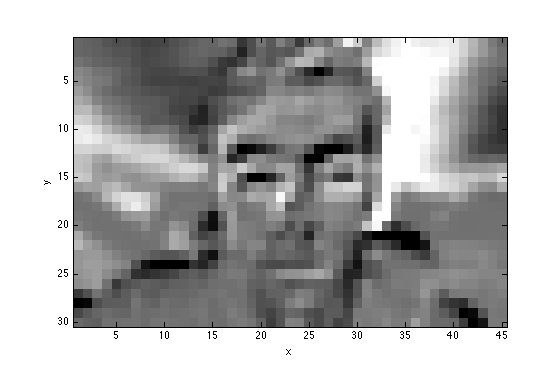
\includegraphics[width=\textwidth]{images/red_peak.png}
      \caption{At at a given time}
    \end{subfigure}
    \begin{subfigure}{.5\textwidth}
      \captionsetup{justification=centering}
      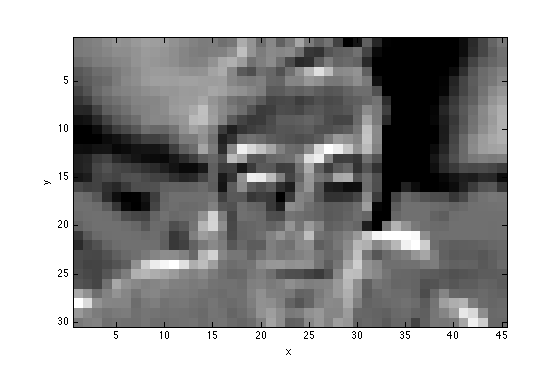
\includegraphics[width=\textwidth]{images/red_trough.png}
      \caption{Half a heartbeat period later}
    \end{subfigure}
    \captionsetup{justification=centering}
    \caption{Red channel of the EVM output, before recombining with the original video.}
  \end{figure}

  What is striking is that the output for these two frames seem like they are the same image with inverted colors. In fact, after processing, the whole video presents a 
  periodic color with a frequency that seems equal to the heartbeat. This does not happen with the data provided in the paper, where in a similar video only the person's face 
  changes color.

  Thus, while the EVM processing strikingly shows that it is possible to extract medically relevant data from a simple video, we also realized that processing had too many 
  unknown effects for us to get started by directly adding new layers on top of it. Thus we decided to start building from the ground up.

  Another question that arose from this visualization was whether or not it would be necessary to use some face detection tool in order to be able to look at the 'right' pixels (those with a heartbeat). We then realized we had actually had a wrong definition of our problem, up until then.

  What we are essentially trying to do is to get the same reading a pulse oximeter, but with a camera.
  An absorbance pulse oximeter essentially measures the absorption of light by a thin layer of tissue through time. Because oxygenated and de-oxygenated hemoglobin do not absorb light at the same wavelength, this measure yields the blood's oxygen saturation, And by measuring the periodic change of absorbance caused by the pulse, the same measure also yields a heartbeat reading.

  Therefore, we could do a mental experiment, measuring pulse oximetry values by placing a pulse oximeter at the physical location of one pixel in our image. Replicating this with a camera thus means that each pixel in our video is a training example. The problem then is not knowing what we are looking at, but getting what colors in our video
  matter for our measurement.

 %%%%%%%%%%%%%%%%%%%%%%%%%%%%%%%
\end{document}


